\documentclass[11pt, a4]{article}
\usepackage{geometry}
\geometry{margin=1.25in}
\usepackage[utf8]{inputenc}
\usepackage[english]{babel}
\usepackage{amsmath}
\usepackage{graphicx}
\graphicspath{ {./figures/} }
\usepackage{placeins}
\usepackage{booktabs}
\usepackage{listings}

\title{Seoul Bike Sharing Demand \\
		\large Supervised Machine Learning: Regression - Course Project}
\author{Caio Mescouto Terra de Souza}
\date{\today}

\begin{document}

\maketitle

\section*{Introduction and Main Objective}

Nowadays rental bikes are a reality in the many urban cities in the world. One of the biggest concerns is maintaining a reliable supply of bicycles to meet public demand regardless of time and weather. However, the demand is not constant. It has, at least, seasonal fluctuation depending where the city is in addition to hourly and weather fluctuations. The maintenance schedule and the logistics of distribution of bicycles between locations are very important due to the fluctuation on demand stated before.

Regarding the main concern presented, the data set I worked on contains the count of public bikes rented at each hour in the Seoul Bike sharing System, besides weather and holiday information. The main objective of this analysis is to build a model highly interpretative where it will be possible to isolate the attributes that are mostly responsible for the demand fluctuation. Even if the goal is interpretation, we would like to avoid underfitting by simplicity and, of course, overfitting by high complexity. I believe that a highly interpretive model is more actionable because it leads to more straight actions that can change certain variables or use this variable in favor of something. In this specific case, a highly interpretative model can lead to improvements on maintenance schedule, for example.

\section*{Data Set Description}

As presented before, the data set contains the count of public bikes rented at each hour in the Seoul Bike sharing System \cite{bike}. It has 14 attributes and 8760 observations. The data set contains one year of data from december, 2017 to november, 2018. The table below summarises the attributes (Table  \ref{table:1}).
 

\begin{table}[h!]
\centering
\begin{tabular}{l c c}
\toprule
\textbf{Column} & \textbf{Dtype} & \textbf{Unit} \\
\midrule
Date & Datetime & year-month-day\\
Hour & int64 & hour\\
Temperature & float64 & Celsius\\
Humidity & int64 & \% \\ 
Windspeed & float64 & m/s \\
Visibility & int64  & 10m\\
Dew point temperature & float64 & Celsius\\
Solar radiation & float64 & MJ/m2\\
Rainfall & float64 & mm\\
Snowfall & float64 & cm \\
Seasons & object & Winter, Spring, Summer, Autumn\\
Holiday & object & Holiday, No Holiday \\
Functional day & object & Non Functional Hours, Functional Hours\\
Rented Bike count & int64 & Count of bikes rented at each hour\\
\bottomrule
\end{tabular}
\caption{Data Set Attributes}
\label{table:1}
\end{table}

\section*{Exploratory Data Analysis (EDA)}

Considering the main objective, the data exploration had 5 steps. First, data cleaning; second, to split the data into train and test data; third, to understand the distribution of the numerical variables; fourth, to analyse the correlation between than and fifth, to understand how the number of rented bikes varies through season and holiday.

Before presenting the steps, some assumptions and limitations have already to be set. The data set is one year long, so, it’s not possible to analyze properly if the demand is increasing or not because the seasonal effect will affect this analysis. Finally, it is assumed the demand for rented bikes is always fully met by the supply, meaning that we don’t have a cut off by scarcity of bikes in any observation. This assumption is needed otherwise the model is biased.

\subsection*{Data Cleaning}

The data set is almost clean, no null, no outliers, no mismatching. The only point is that the variable \textit{Functional day} flags whether the service is operational or not and, as we are interested in the demand, we can drop all no operational observations ($295$ entries) that represent only $3\%$ of the data set.

\subsection*{Data Stratified Sampling}

To avoid hacking the model it is important to split the data between train and test data as early as possible. Just after the first view and the data cleaning, the data was split using a stratified split. The stratification followed the distribution of the target variable (\textit{Rented Bike Count}) whitin 5 bins and the test set was set in $20\%$ of the data. Below the \textit{Scikit-Learn} implementation applied.

\begin{lstlisting}
StratifiedShuffleSplit(n_splits=1, test_size=0.2, random_state=0)
\end{lstlisting}

\subsection*{Numerical Variables}

This subsection covers two steps of the EDA plan (third and forth). First the histograms of all numerical variables were plotted and two problems that can interfere in modeling were spotted. First, some variables are far away from normal distributions, second the scale is also different between them. The scaling was tackled during the data preparation process that precedes the modeling process. The distribution of the target value is presented below as well as the data treatment (Figure \ref{fig:hist_target}). After analyzing the skewness of all numerical variables (Table \ref{table:2}) A log transformation was applied whenever skewness was greater than $0.4$. 

\begin{figure}[!h]
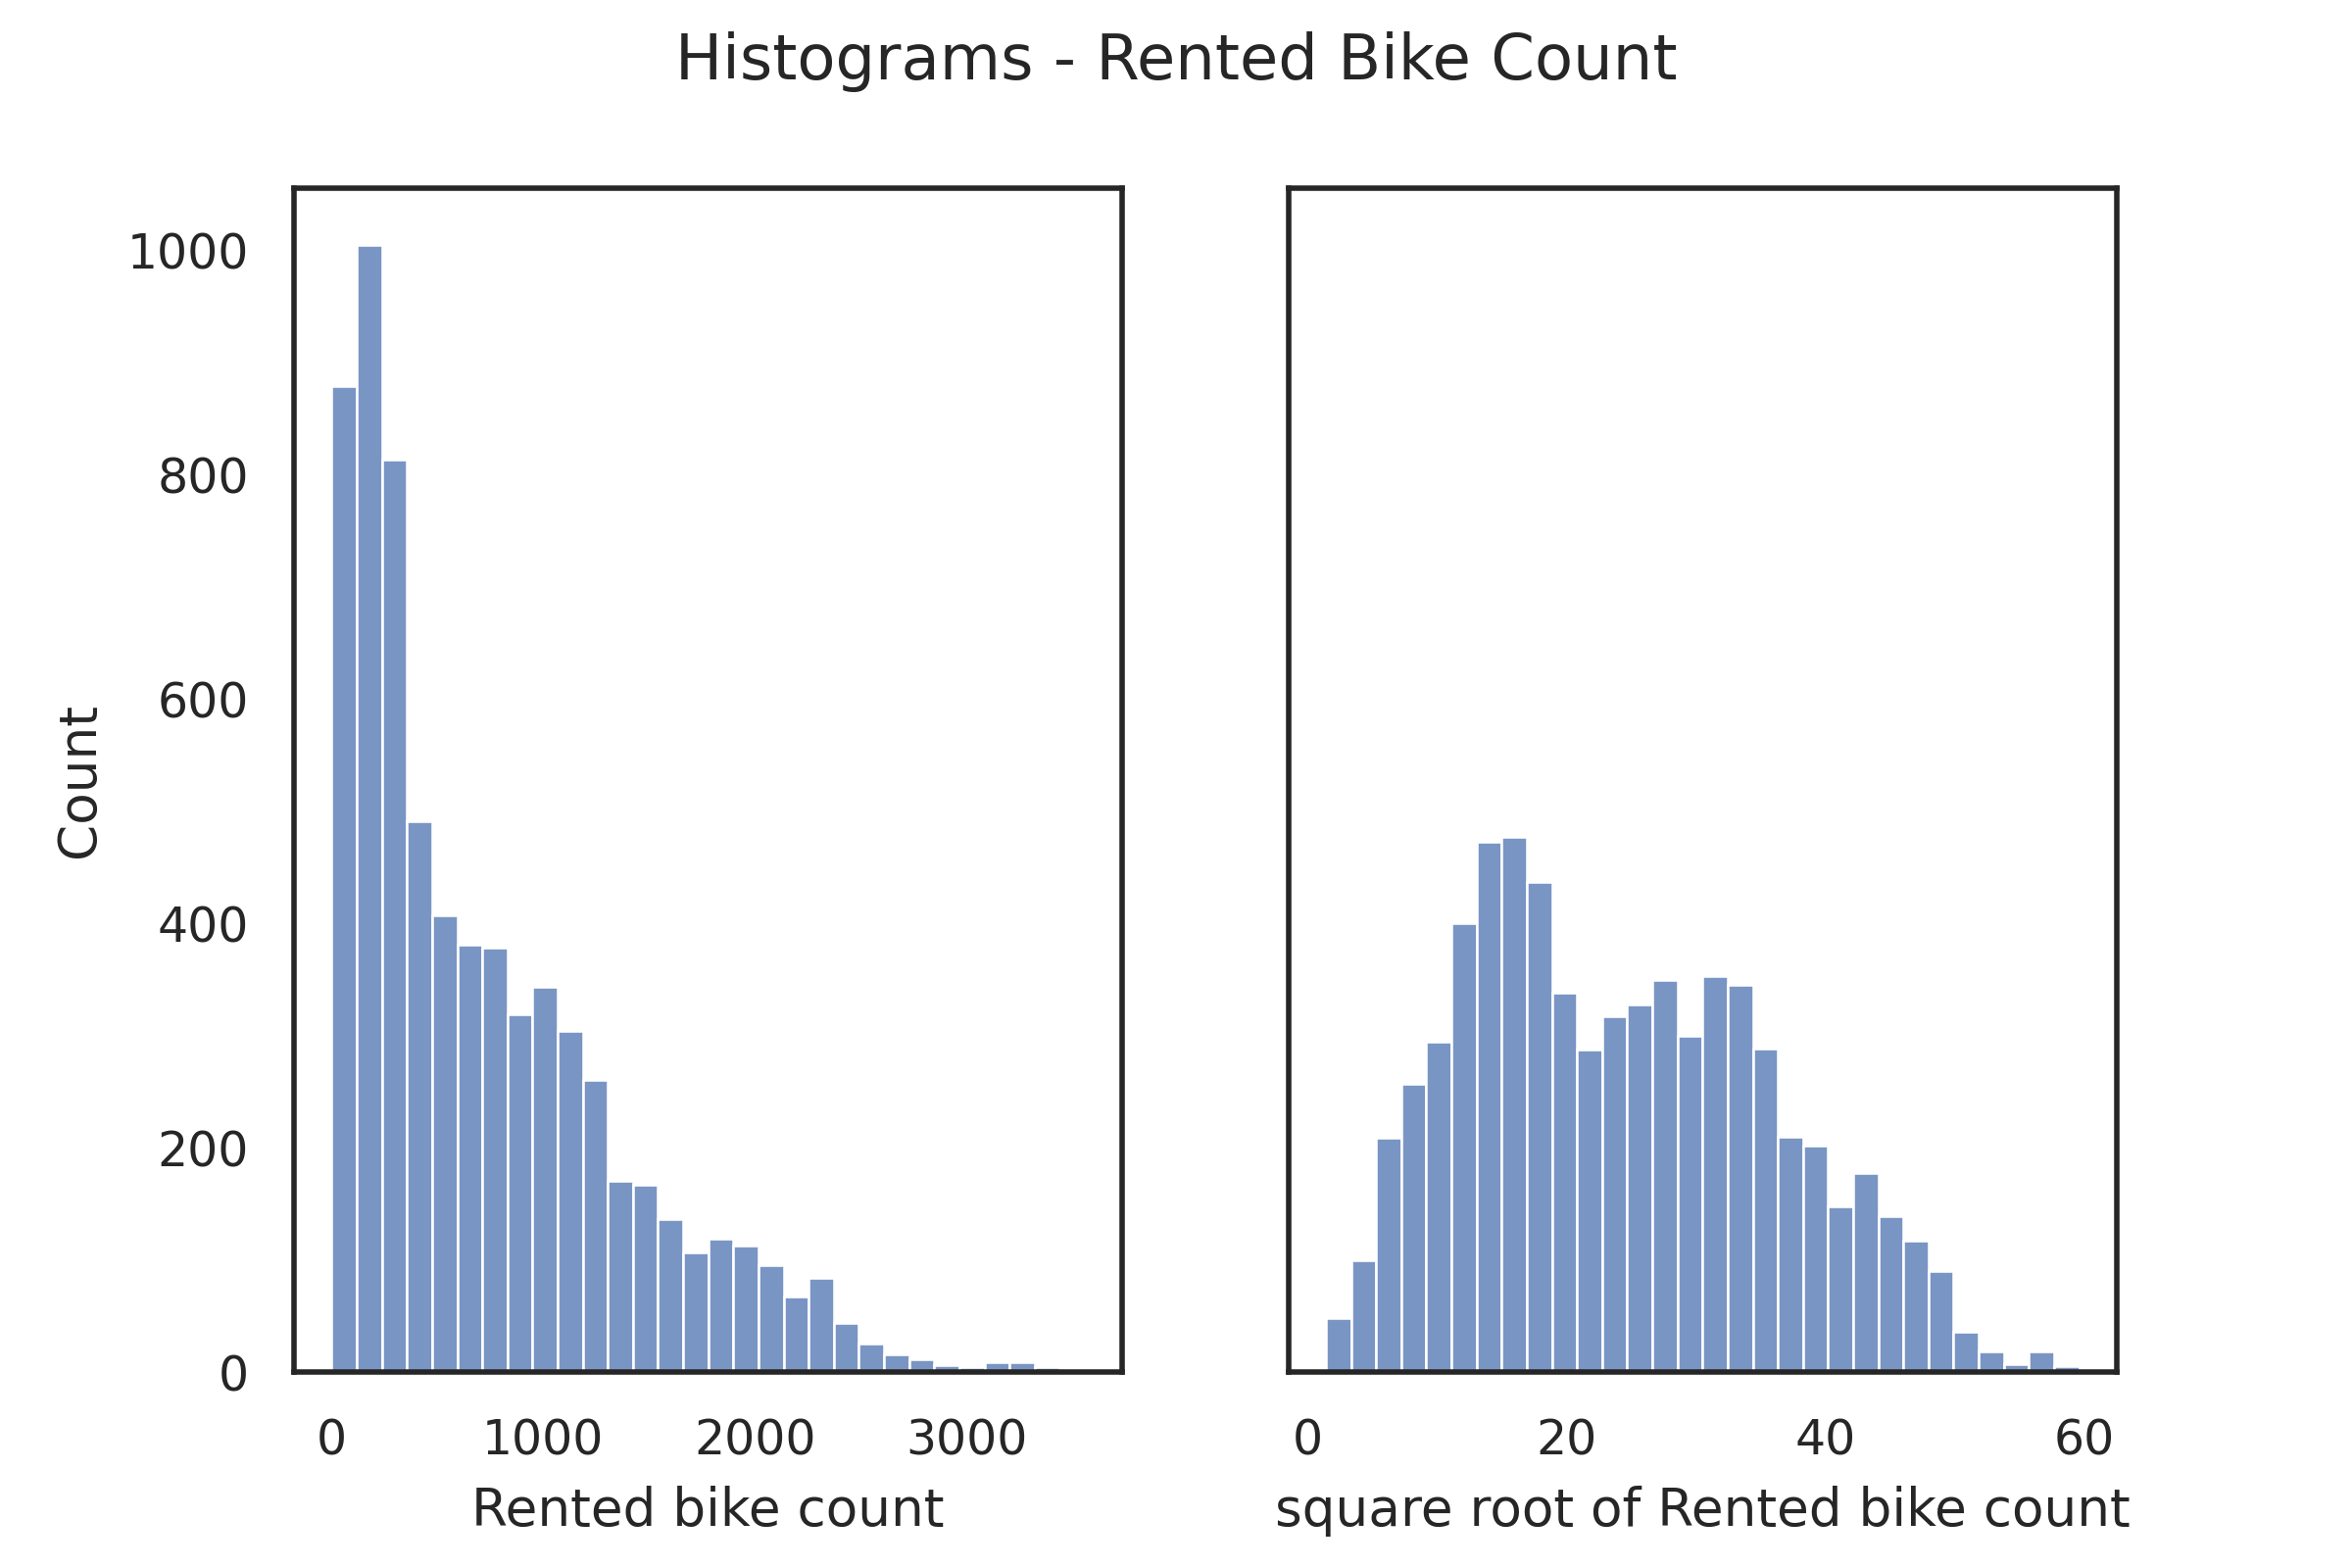
\includegraphics[]{hist_target}
\centering
\caption{Target Histograms}
\label{fig:hist_target}
\end{figure}


After those transformations, the correlation between all variables (including the transformations) was carried out. In general was observed a improvement in correlation comparing the orignal variables and the transformations.

\begin{table}[h!]
\centering
\begin{tabular}{l c c}
\toprule
\textbf{Column} & \textbf{Skewness} \\
\midrule
Hour & $-0.0025$\\
Temperature & $-0.1775$\\
Humidity & $0.0704$\\ 
Windspeed & $0.9126$\\
Visibility & $-0.6964$\\
Dew point temperature & $-0.3394$\\
Solar radiation & $1.5026$\\
Rainfall & $14.2689$\\
Snowfall & $7.8840$ \\
\bottomrule
\end{tabular}
\caption{Data Skewness}
\label{table:2}
\end{table}

Variables that are highly correlated with each other should be avoided due to collinearity issues. As we can observe in the heatmap below (Figure \ref{fig:heatmap}), all variable transformations have highly correlation with the original one, as the correlation with the target was improved through the transformations, we dropped all originals in favor of the transformation. Finally, \textit{Dew point temperature} has high correlation with \textit{Temperature}, as the last one is more correlated with the target, it will be keeped and the former one will be dropped.




\begin{figure}[!h]
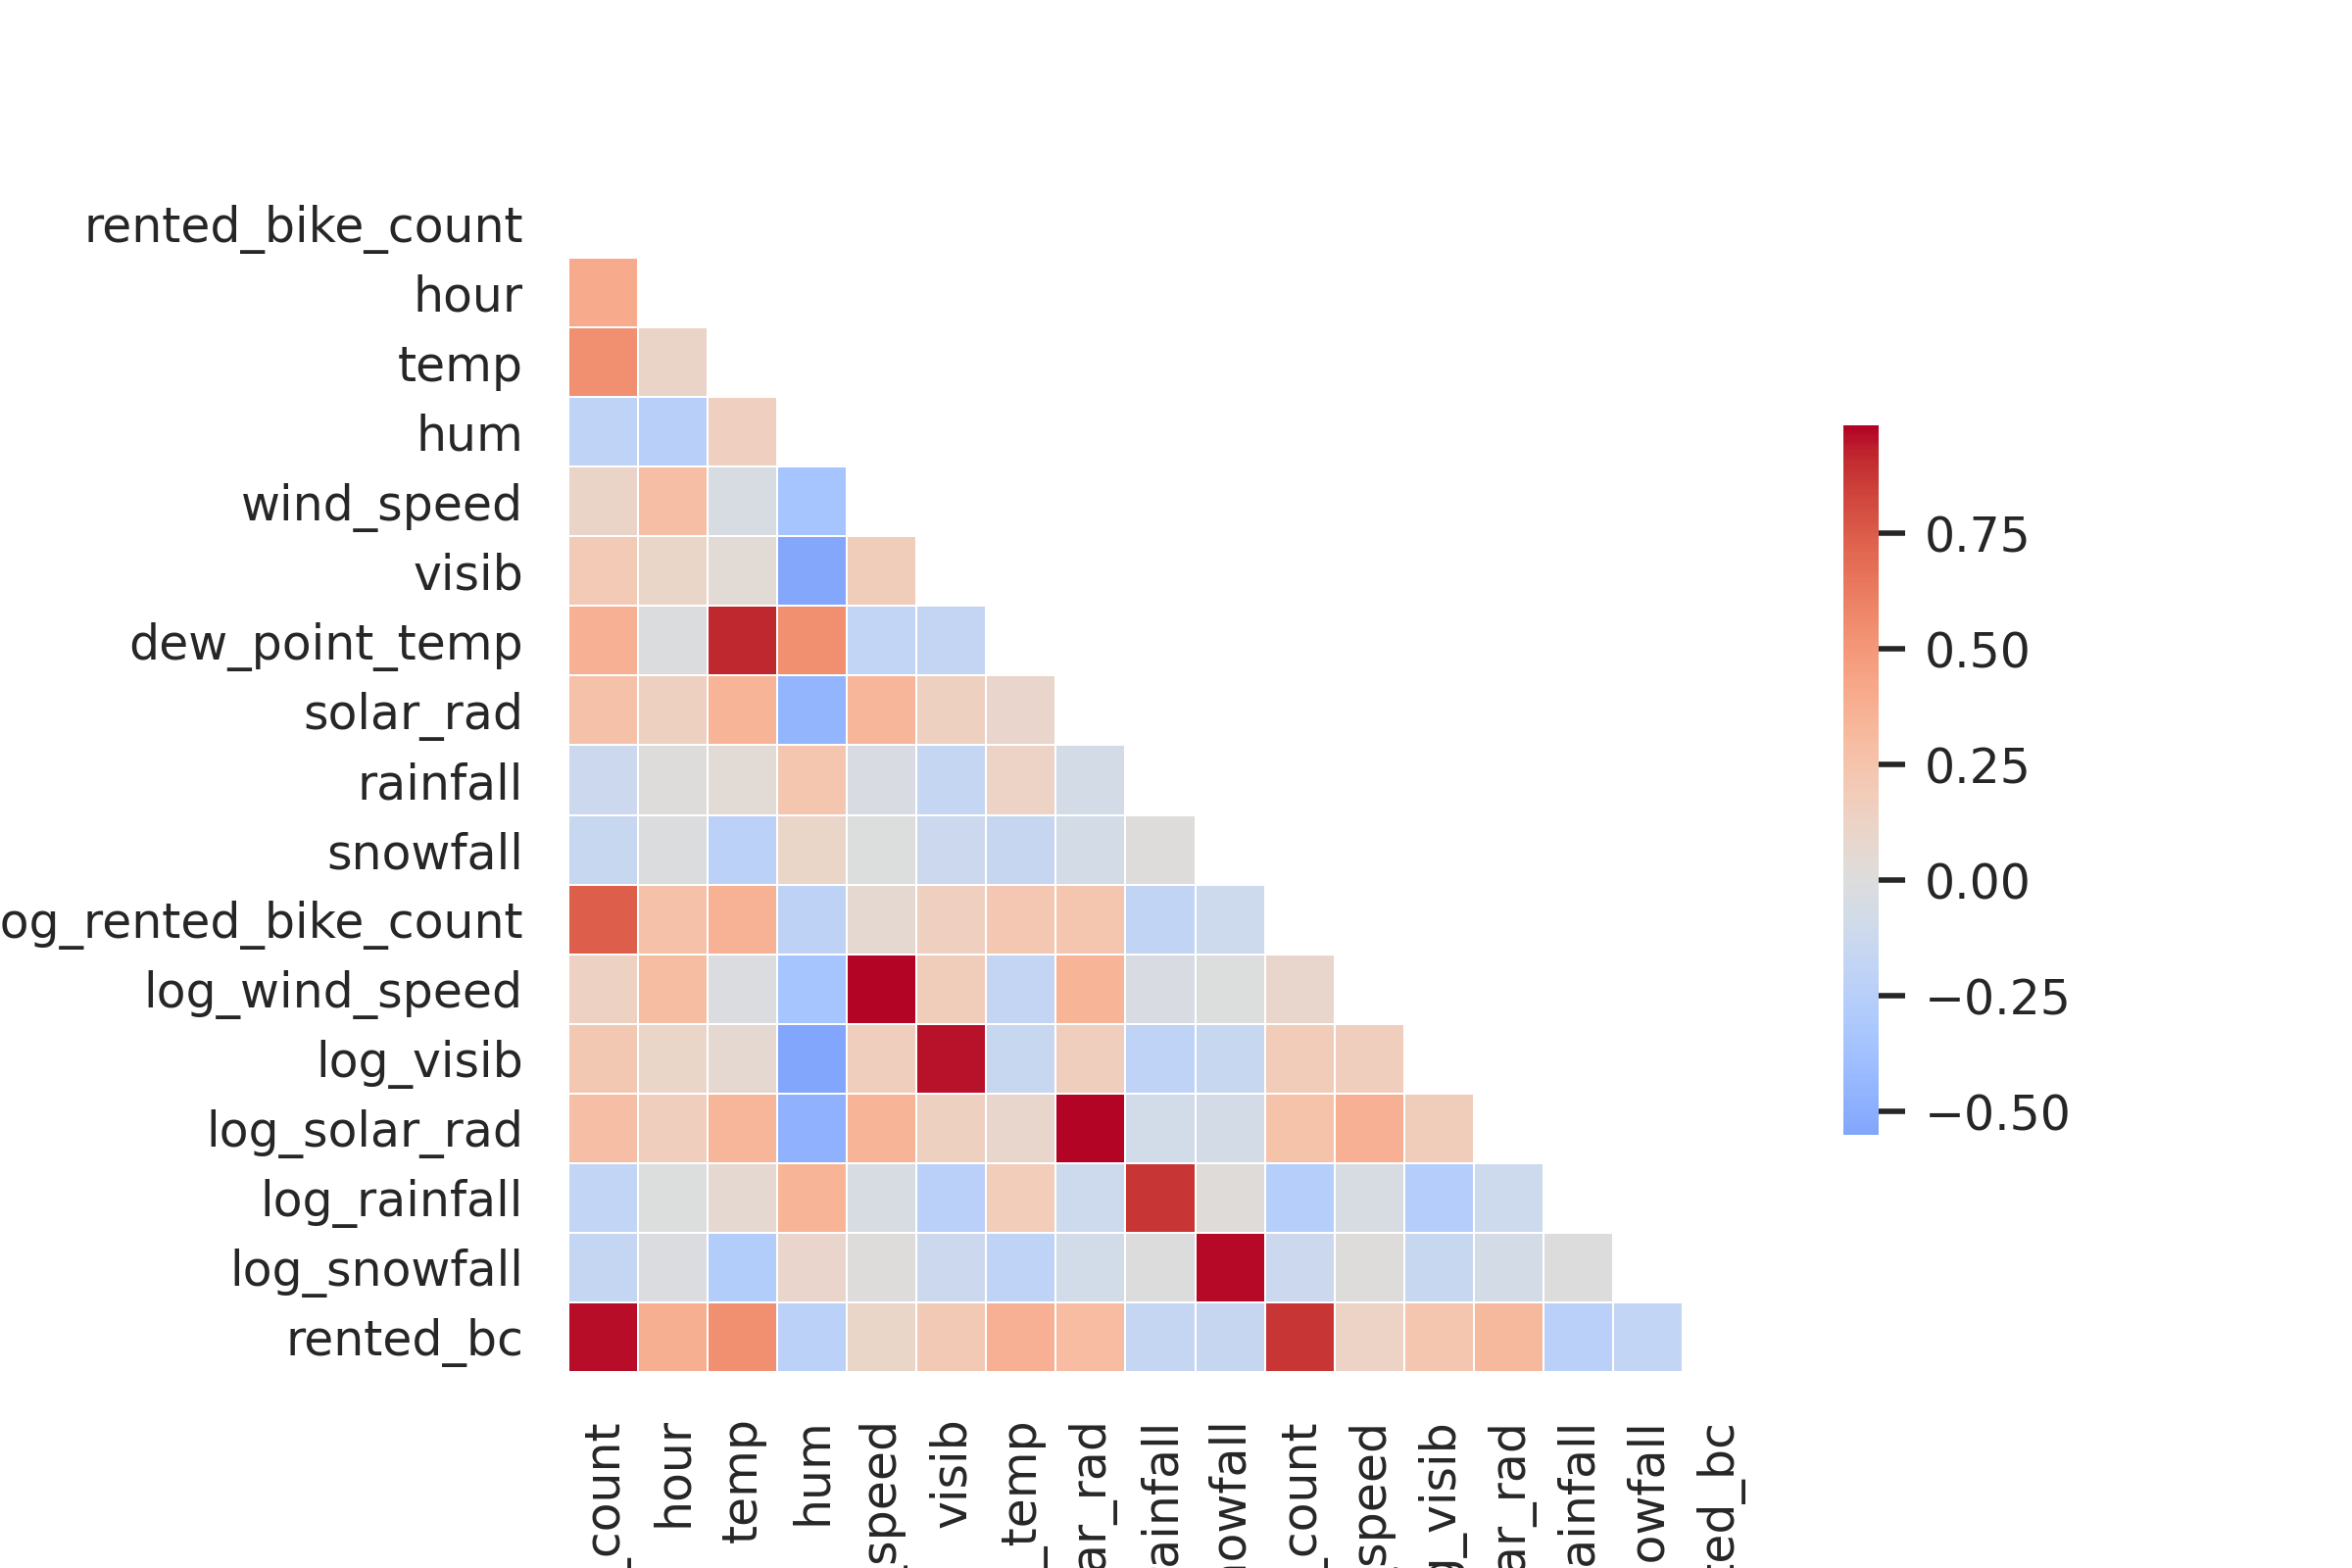
\includegraphics[]{heatmap}
\centering
\caption{Heatmap of correlations}
\label{fig:heatmap}
\end{figure}


\subsection*{Categorical Variables}

The last phase of the EDA is to analyze the relationship between the target value and the categorical variables. According to the violin plot (Figure \ref{fig:violin}) below we can easily observe that \textit{Winter} is the season when the bikes are less rented and during this season, those who ride a bike do it more as means of transportation, because \textit{No Holiday} has higher demand than \textit{Holiday}. During the \textit{Spring} the demand, in general, is higher than during \textit{Winter}, but the same pattern is observed (\textit{No Holiday}$>$\textit{Holiday}). \textit{Autumn} and \textit{Summer} have the average greater than \textit{Winter} and \textit{Spring} and are quite similar between them both, with no strong pattern between \textit{Holiday} and \textit{No Holiday}. These patterns are expected due to the difference of temperature and rainfall/snowfall. But for me it was interesting to observe these differences between \textit{Holiday/No Holiday}.
 

\begin{figure}[!h]
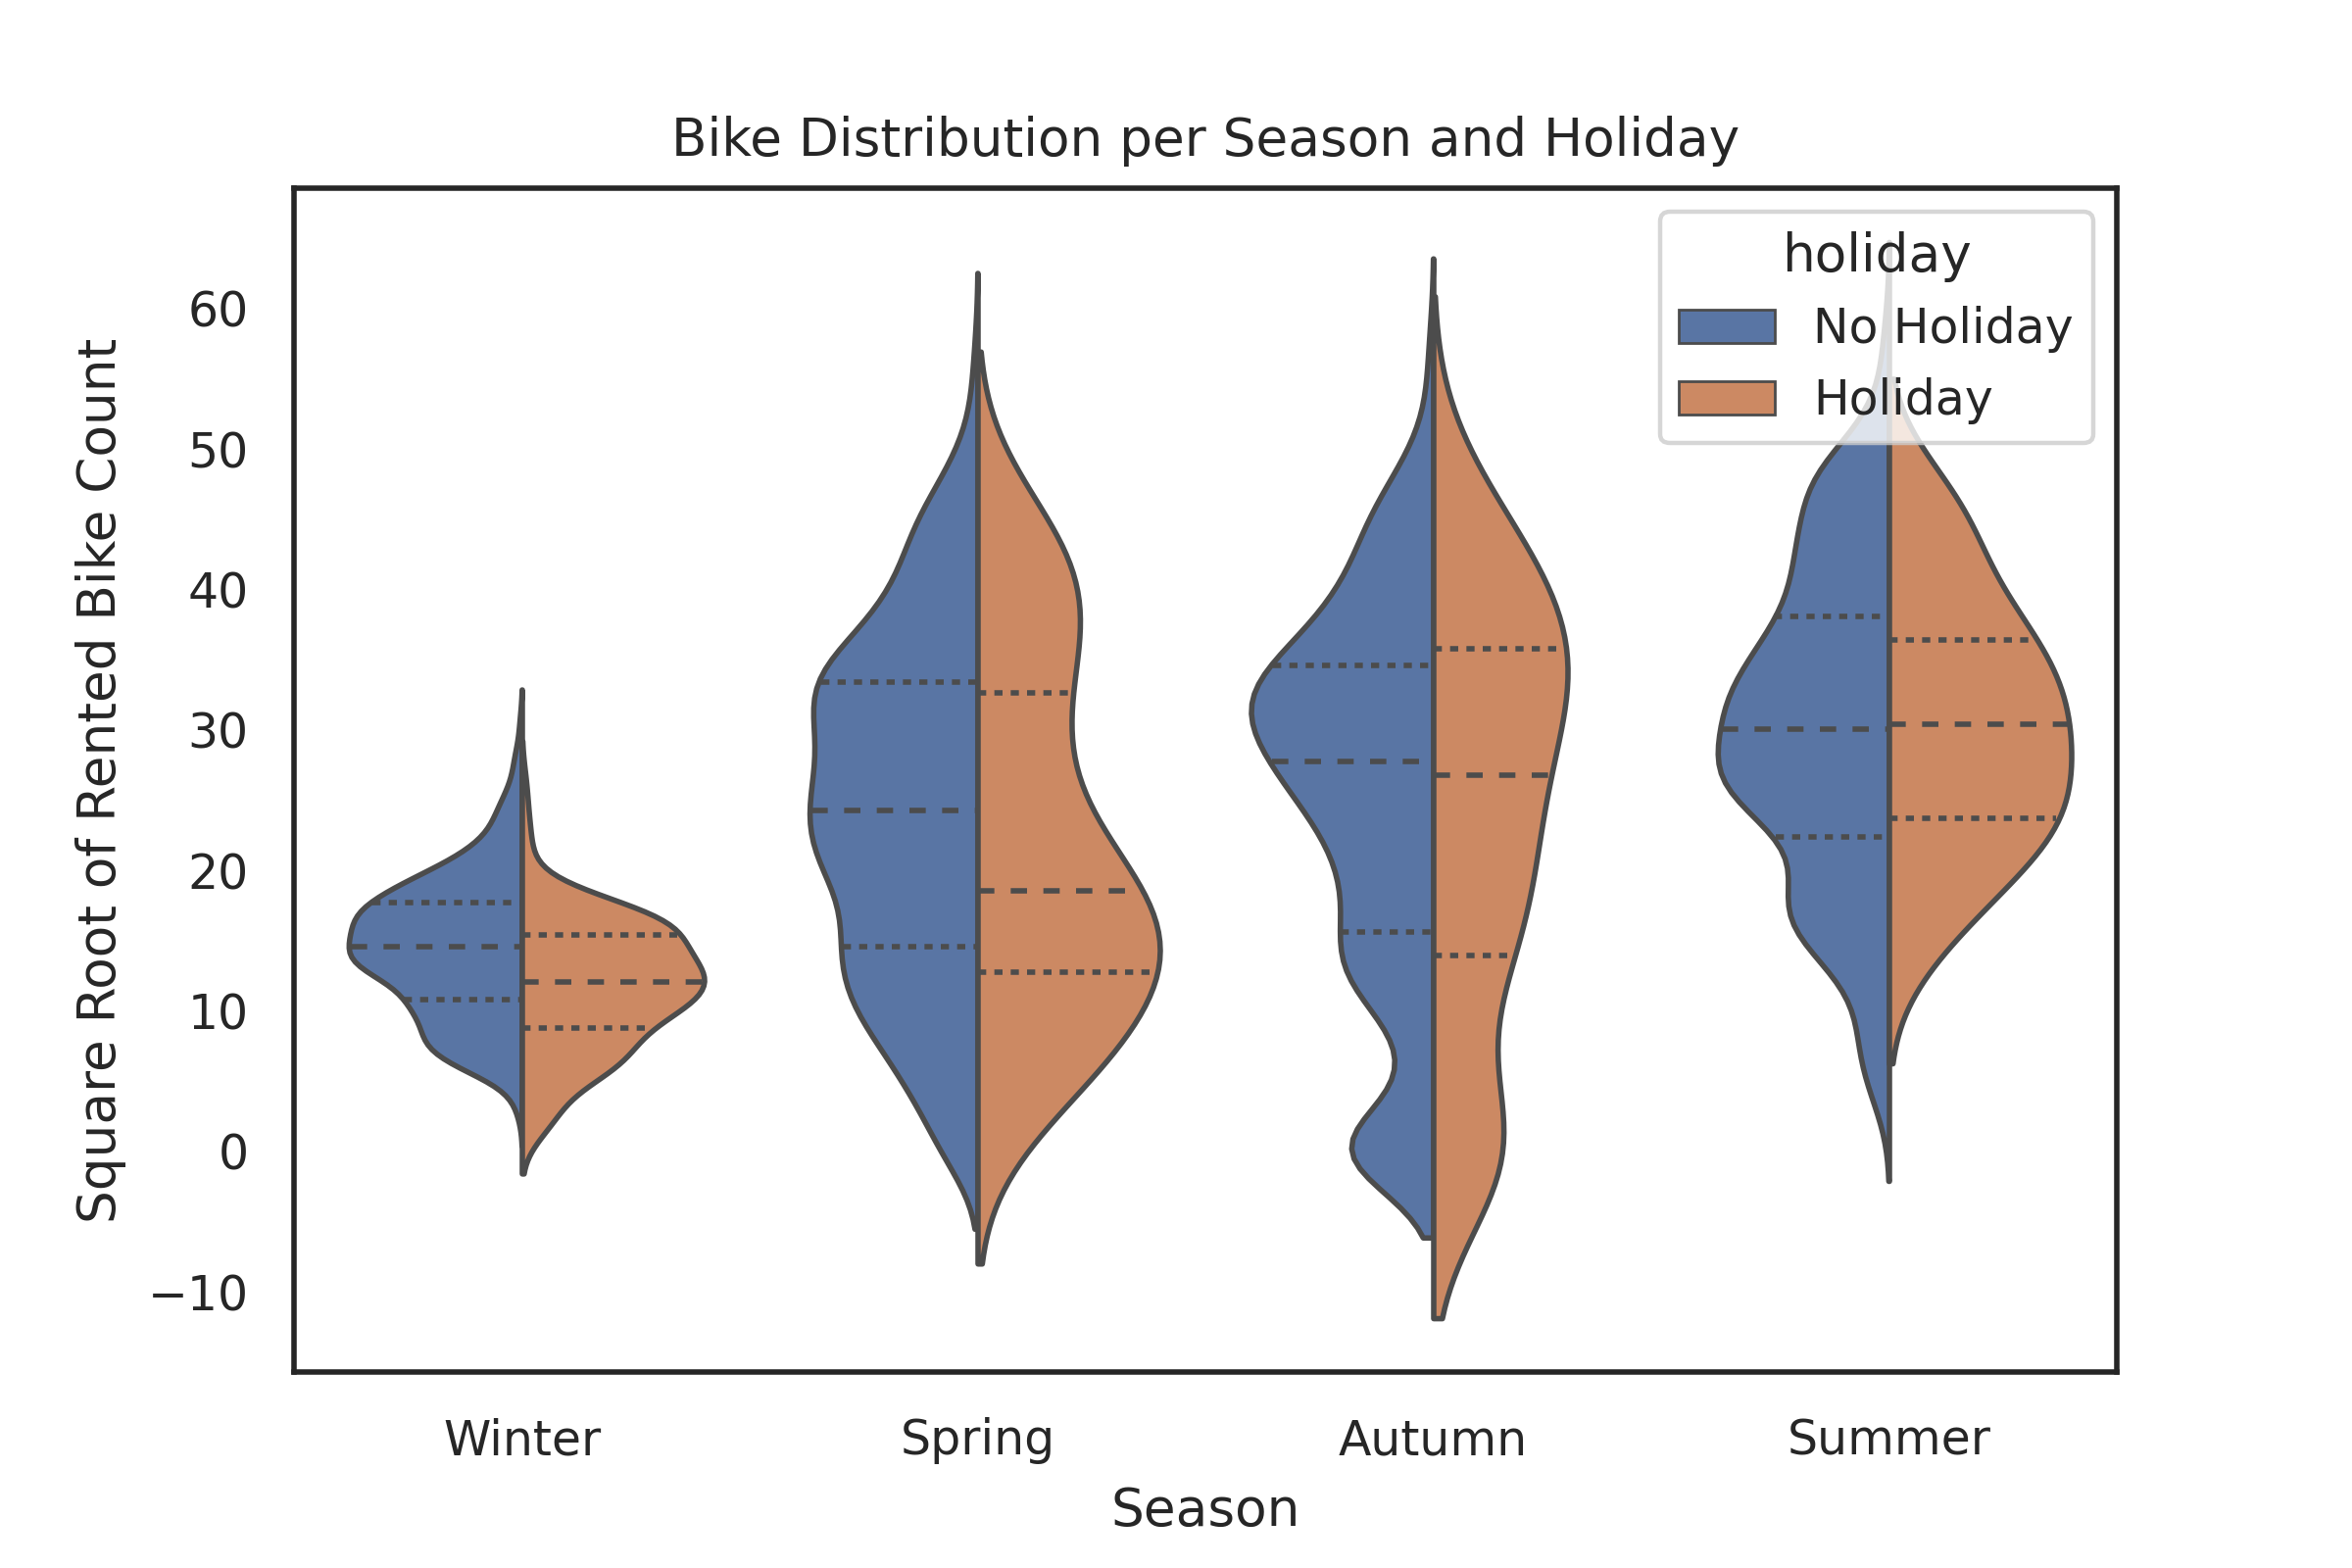
\includegraphics[]{violin}
\centering
\caption{Bike Distribution per Season and Holiday}
\label{fig:violin}
\end{figure}

\section*{Data preparation and Feature Engineering}

Some of the features engineering applied were already covered in the previous section. This section presents only the step by step used to prepare the data for modeling.

\begin{enumerate}
\item Split the data into train and test data set;
\item Filter the data only where \textit{Functional day} is True;
\item Drop \textit{Functional day, Date, Dew point temperature};
\item Data log transformation in \textit{Windspeed, Solar radiation, visibility, rainfall, snowfall};
\item Divide data set into Features and Target;
\item Data Square root transformation in Target value;
\item Scale numerical variables with \textit{Scikit-Learn}
\begin{lstlisting} 
StandardScale() ;
\end{lstlisting}
\item Encode categorical variables with \textit{Scikit-Learn}
\begin{lstlisting} 
OneHotEncoder(drop='first') .
\end{lstlisting}
\end{enumerate}

\section*{Model Selection}

As stated in the first section, our main objective is to set up a model as simple as possible that fits the data, but where we can understand how the target is affected by the features. This model should avoid both under and overfit and have as few variables as possible. This problem is complicated because the number of variables is high related to under and overfitting. Therefore, first the $R^2$ was chosen as a parameter to compare models, as it is a measure of how well the model fits the data (or explains the phenomenon).
The last concern is to ensure generalization (which is an overfitting concern as well), so a cross-validation model for training models should also be adopted. the Below is presented the step by step of this selection and further explanations.

\subsection{Cross-Validation}

All simulation during the model selection used the same set up for cross-validation:

\begin{lstlisting} 
GridSearchCV(<model>, n_jobs=-1, param_grid=<model parameters>, 
scoring='r2', return_train_score=True)
\end{lstlisting}

\subsection{Models}

Four models were shortlisted as follow:

\begin{lstlisting} 
LinearRegression()
Lasso(random_state=0, max_iter=10000)
ElasticNet(random_state=0, max_iter=10000)
OrthogonalMatchingPursuit()
\end{lstlisting}

The most simple is the \textit{Linear Regression} and it is likely to underfit the data. To avoid underfitting the data we first used this model to set the optimum degree for the polynomial features. As high polynomial degrees, on the other hand, tend to overfit the data, the cross validation was applied to avoid the other extreme as well. The \textit{Polynomial Features} was optimized as follow. It's also import to highlight that small degree is consistent with more interpretability.

\begin{lstlisting}
PolynomialFeatures(degree=3, include_bias=False)
\end{lstlisting}

After the optimization three other models were selected to improve the fitness through regularization. The \textit{Lasso} regression throughout $\ell_1$ penalization tends to force some coefficients to zero and this is more prominent with $\ell_1$ penalization than $\ell_2$ penalization (\textit{Ridge}). Despite the computational superiority of the \textit{Ridge regression}, the data set is relatively small and we are more interested in interpretability, so we picked \textit{Lasso}. However, as we are also interested in a goodfit, we also set up a \textit{ElasticNet} that combines both penalties ($\ell_1\: and\: \ell_2$) and we can weight these penalties. The last model is the \textit{Orthogonal Matching Pursuit (OMP)} implements the OMP algorithm for approximating the fit of a linear model with constraints imposed on the number of non-zero coefficients (ie. the $\ell_0$ pseudo-norm) \cite{OMP}. As we are interested in the fewest possible Features and this model is highly efficient in computational terms, it is a good candidate.

\subsection{Cross-validation results}

 \begin{table}[h!]
\centering
\begin{tabular}{l c c}
\toprule
\textbf{Best Estimator} & \textbf{$R^2$} \\
\midrule
LinearRegression(normalize=True) & $0.7943$\\
Lasso(alpha=0.0060, max\_iter=10000, random\_state=0) & $0.8153$\\
ElasticNet(alpha=0.0060, l1\_ratio=1.0, max\_iter=10000,
            random\_state=0) & $0.8153$\\ 
OrthogonalMatchingPursuit(n\_nonzero\_coefs=155) & $0.8144$\\
\bottomrule
\end{tabular}
\caption{Cross-Validation Results}
\label{table:3}
\end{table}

Following this result it is possible to infer that \textit{Lasso} fits better than \textit{Ridge} in this data set, as the best estimator with \textit{ElasticNet} is in reality the same of \textit{Lasso} ($\ell_1ratio=1$). In brief all estimators had achieved good scores. However, as we are interested in interpretability we dropped the linear regression and will further investigate \textit{Lasso} and \textit{OrthogonalMatchingPursuit}.


\section*{Model Interpretation and Key Findings}

Two simple ways to start analysing complexity is to understand the weights and the number of non-zero coefficients. In addition to the $R^2$, Lasso is a also more simple model than OrthogonalMatchingPursuit (Table \ref{table:4}).

 \begin{table}[h!]
\centering
\begin{tabular}{l c c c}
\toprule
\textbf{Model} & \textbf{Coefficients} & \textbf{$=0$} & \textbf{$\sum{|\text{coefficients}|}$} \\
\midrule
Lasso & $168$ & $28$& $126.0955$\\
OrthogonalMatchingPursuit & $168$ & $13$ & $154.2423$\\
\bottomrule
\end{tabular}
\caption{Models Coefficients}
\label{table:4}
\end{table}

Although these measures of complexity, interpretation means to understand which variables are more responsible and in which direction they affect the target value. Below (Table \ref{table:5}) are presented the 10 more important variables with their respective coefficients for each model and the key insights. For sanity it's not repeated log all the time but \textit{Rainfall and Solar Radiation} are in fact, log transformed.


 \begin{table}[h]
\centering
\begin{tabular}{l c |c c}
\toprule
\textbf{Lasso} & \textbf{Coef.} & \textbf{OrthogonalMatchingPursuit} & \textbf{Coef.} \\
\midrule
$hour^2\times solarRad$ & $10.5964$ & $rainfall$& $-12.4247$\\
$hour\times solarRad$  & $-10.3316$ & $hour^2\times solarRad$ & $11.1473$\\
$rainfall$ & $-10.2103$ & $hour\times solarRad$ & $-10.9250$ \\
$hour^2$ & $8.3205$ & $hour^2$ & $8.8413$ \\
$temperature$ & $6.8650$ & $temperature$ & $7.3074$ \\
$winter$ & $-6.2208$ & $winter$ & $-6.3295$\\
$solarRad^2$ & $-3.8585$ & $solarRad^2\times rainfall$ & $4.7297$ \\
$hour^3$ & $-3.6222$ & $solarRad^2$ & $-4.1108$ \\
$spring$ & $-3.4217$ & $hour^3$ & $-3.7492$ \\
$solarRad^2\times rainfall$ & $3.3945$ & $spring$ & $-3.6187$ \\
\bottomrule
\end{tabular}
\caption{Main Features}
\label{table:5}
\end{table}

\subsection*{Key Findings}

\begin{itemize}
\item First of all, It is interesting that all variables are the same, with differing intensities but Lasso always has smaller coefficients than OrthogonalMatchingPursuit, meaning that Lasso is probability more regularezed than  OrthogonalMatchingPursuit;
\item Almost half of the most important variables has degree equal 3, meaning that the polynomial transformation played a important role in fitting the model;
\item Only five of the eleven variables are listed in the top 10 (\textit{Hour, Solar Radiation, Precipitation, Temperature, Season});
\item \textit{Rainfall} has a negative effect on the target, but combined with the power of \textit{Solar Radiation}, this effect is positive. As the power itself has a negative effect, Usually  days with a little bit of rain but sunny are normal in the summer and the temperature is high.
\item \textit{Hour} has different effects on the target, below it is a plot of the mean demand per hour that can help understand this erratic behavior (Figure \ref{fig:rented}).
\end{itemize}

\begin{figure}[!h]
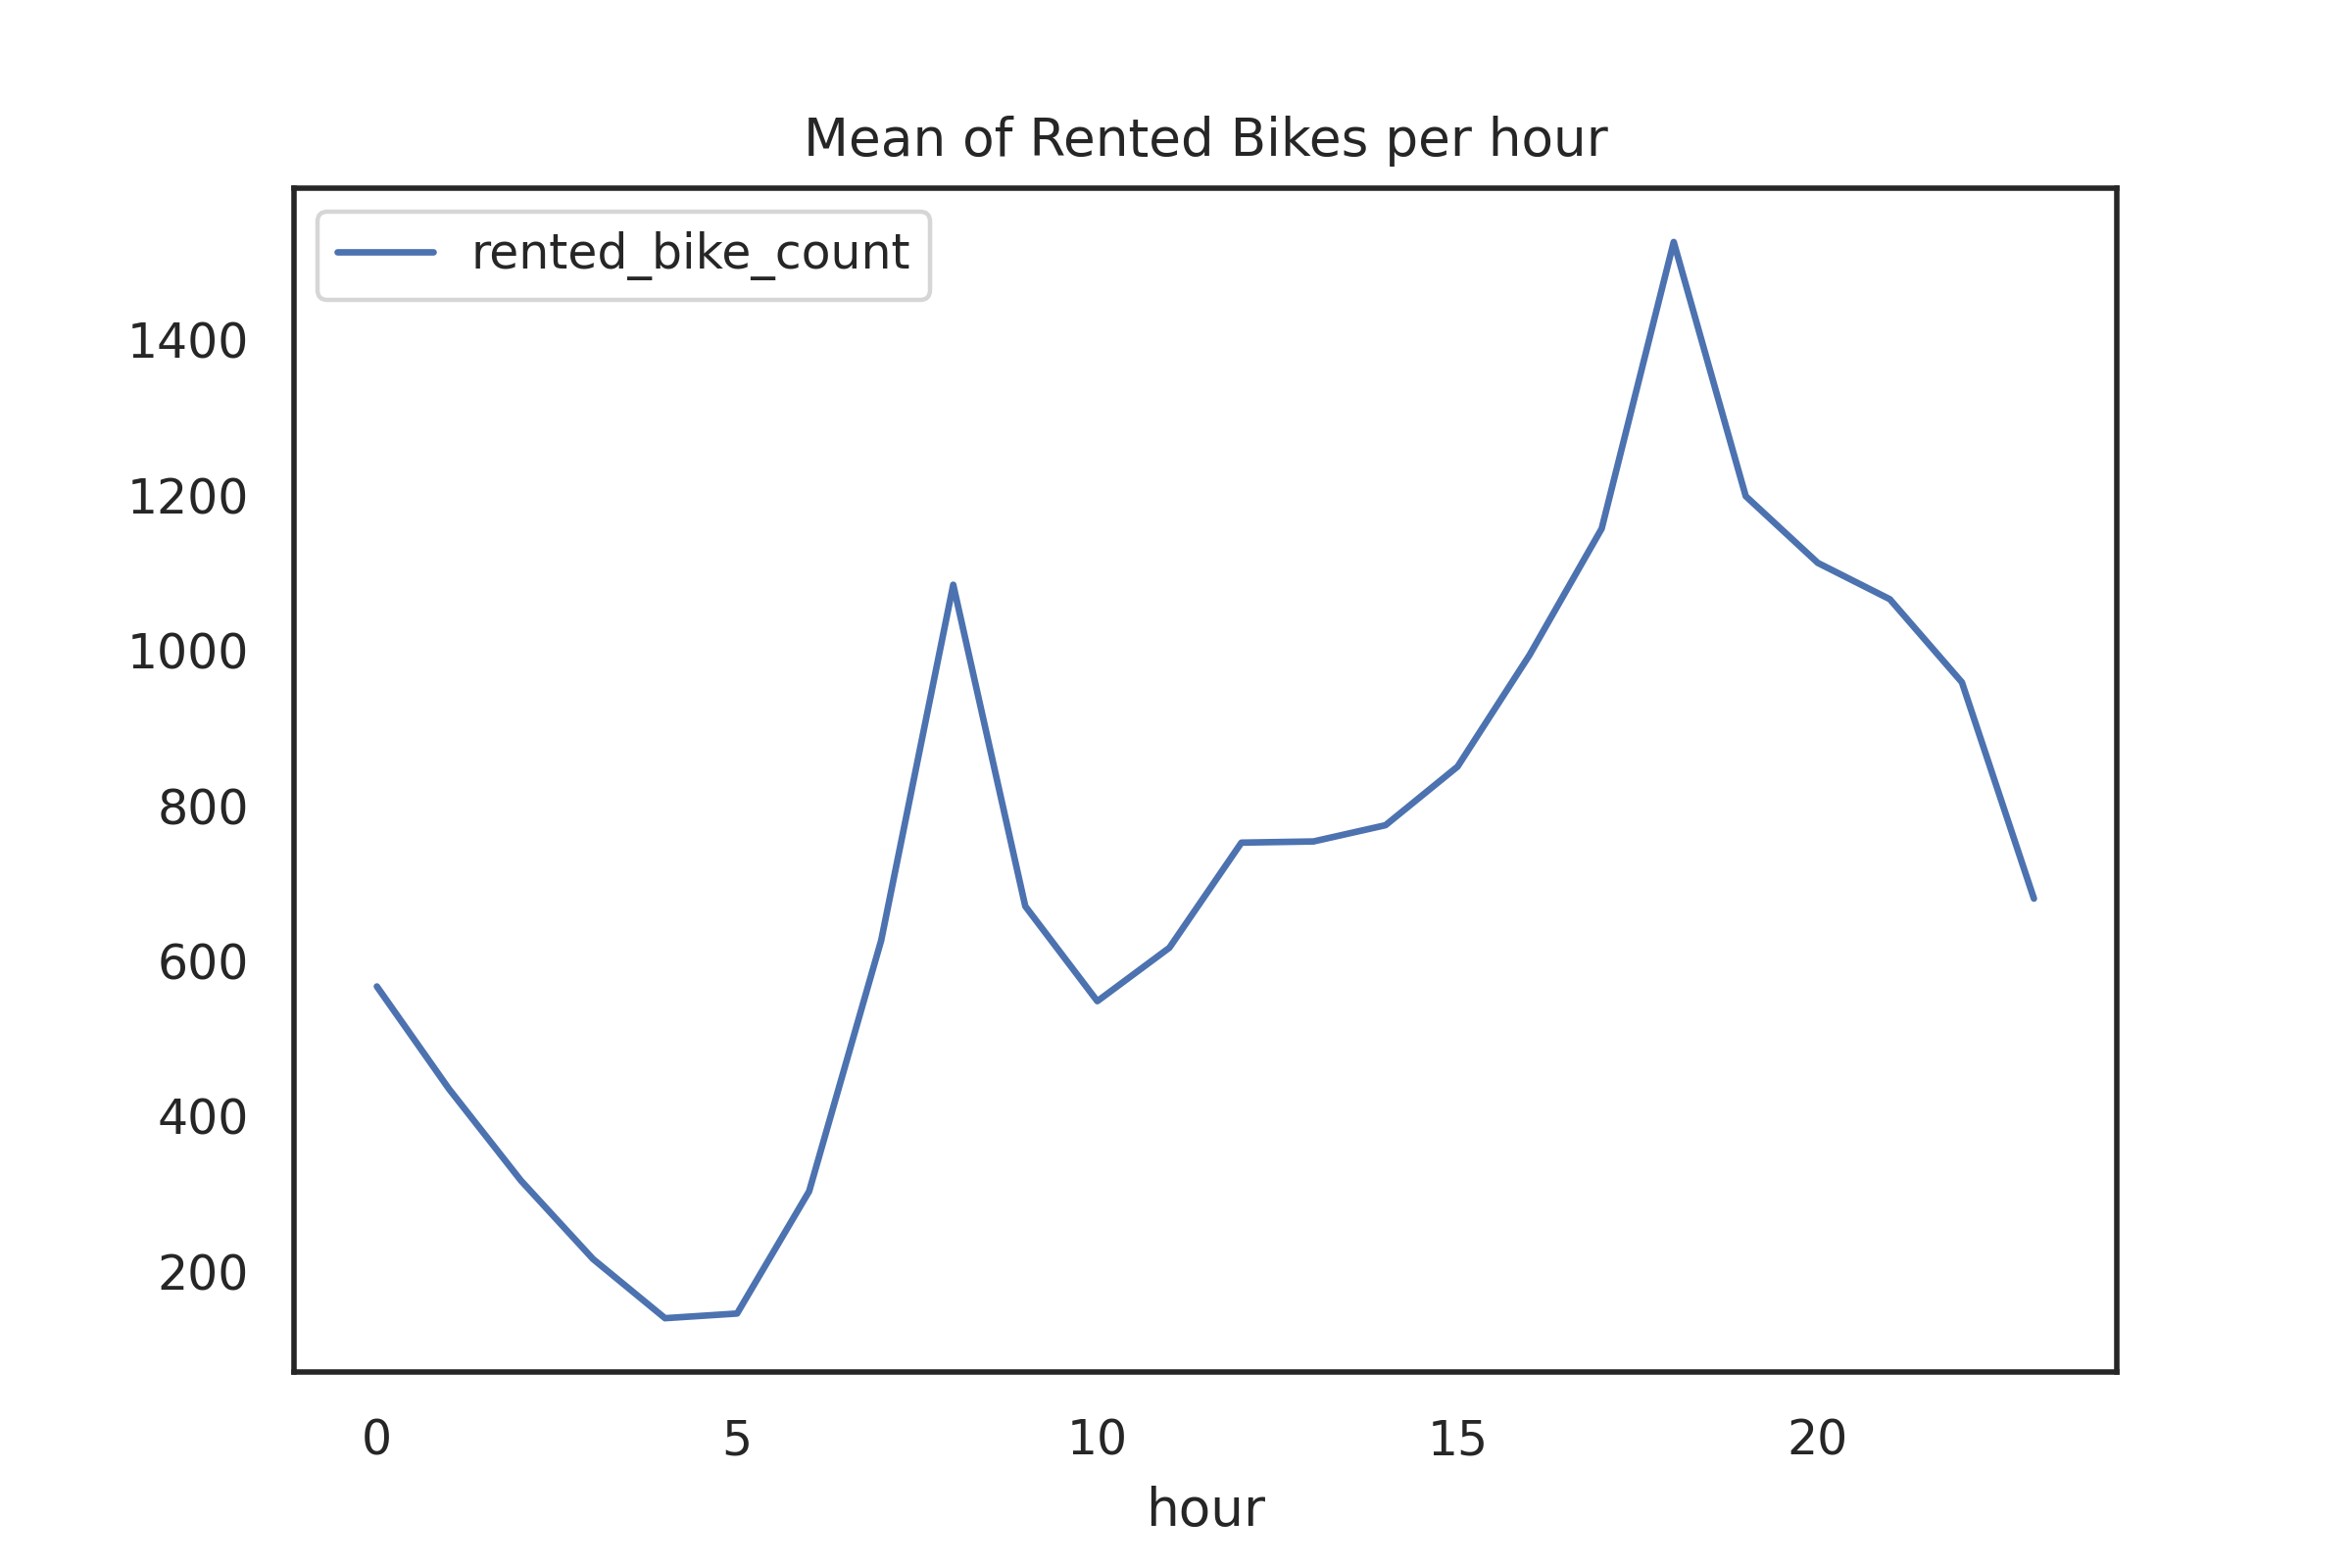
\includegraphics[]{rented}
\centering
\caption{Mean of Rented Bikes per hour}
\label{fig:rented}
\end{figure}


\subsection*{Test set}

The last phase before choosing a model and presenting the conclusion is that both models were tested against the test data set and the result is presented below (Table \ref{table:6}).

\begin{table}[h!]
\centering
\begin{tabular}{l c c c}
\toprule
\textbf{Model} & \textbf{$R^2$} \\
\midrule
Lasso & $0.8156$ \\
OrthogonalMatchingPursuit & $0.8118$\\
\bottomrule
\end{tabular}
\caption{Models performance}
\label{table:6}
\end{table}

\section*{Model selection}

Both models had performed as good as during the cross-validation, meaning that under and overfitting were both avoided. Finally, The \textit{Lasso} regression is suggested to be adopted. The performance is better and interpretation-wise there is no difference in terms of top 10 variables, but has small coefficients and more zero-coefficients.

\section*{Next steps and Improvements}

The main flaw of the model is the granularity of the data. It is not a microdata that has information like localization of the bike or the time spent in the ride. This information would be used to improve the model, for example, connecting the flux of bikes during the period of the day or, understanding if some bikes spots are overloaded. These data should have granularity about weather as well, for example sparsity of the rain or solar radiation in different locations.



\FloatBarrier

\begin{thebibliography}{9}

\bibitem{bike} 
Seoul Bike Sharing Demand Data Set,
\\\texttt{https://archive.ics.uci.edu/ml/datasets/Seoul+Bike+Sharing+Demand}

\bibitem{OMP}
1.1.9. Orthogonal Matching Pursuit (OMP),
\\\texttt{https://scikit-learn.org/stable/modules/linear\_model.html\#omp}
\end{thebibliography}

\end{document}